%\part{title}
\chapter{Introducción}
%\label{chapter:introduction}

%\begin{introduction}
Desde tiempos de antaño el hombre se ha visto en la necesidad de manejar, de la manera más adecuada posible, sus recursos; no solo para conseguir prolongar la vida de estos, sino además para contar con una aceptada utilización de los mismos. Uno de los principales problemas que aqueja a la sociedad actual es la dificultad que se presenta para garantizar un óptimo manejo de nuestro \textit{tiempo}.\cite{bbc_time_management}
	
La denominada \textit{gestión del tiempo} hace referencia a la forma en que cada uno organiza y planifica cuánto invierte en actividades específicas. En muchos escenarios cotidianos, a la planificación de las actividades no se le ofrece demasiada atención y esta es manejada a la ligera; por otro lado, existen ámbitos donde se hace necesario garantizar una manipulación detallada de todo el proceso.
	
Con la llegada de las tecnologías actuales y la facilidad con que las personas cambian de actividad, el desarrollo de un software que garantice una planificación de nuestra agenda diaria, resulta casi imprescindible.
	
Un ejemplo claro donde sin duda se comprueba el proceso antes expuesto, es la gestión de las actividades de un centro de estudios y más aún en esta época donde contamos con grandes instituciones universitarias que albergan a cientos de estudiantes con diferentes planes de trabajo y manejan un número considerable de recursos y útiles.
	
La confección de un horario para una institución universitaria puede llegarse a considerar como algo sencillo, pero cabe destacar que la persona encargada de dicha labor, emplea un valioso tiempo en esto; puesto que hay que preveer que no existan colisiones entre los turnos, los locales, los profesores, además de garantizar que todas las actividades se realicen con la frecuencia que corresponde para garantizar el aceptado desarrollo del proceso de aprendizaje por parte del estudiantado.
	
Resulta llamativo como varias universidades cubanas hoy en día aún no cuentan con un sistema propio (o de terceros) para realizar las tareas de confección del horario; sino que en la mayoría de los casos usan softwares como \textit{Microsoft Excel} para gestionar el mismo; lo cual, sin lugar a dudas es sumamente ineficiente y genera un esfuerzo extra para la persona que está desarrollando el mismo, quién sin lugar a dudas debe tener otra serie de tareas que requieran de más importancia.
	
El trabajo en cuestión persigue presentar un software para proporcionar un sistema que permita manejar el sistema de turnos de clases de la \textit{Facultad de Matemática y Computación} de \textit{La Universidad de La Habana}.
	
\section{Motivación}
Desde hace poco más de 10 años en la Facultad de Matemática y Computación se ha venido gestado la idea de presentar un modelo de horario propio que sea capaz de satisfacer las necesidades internas de la misma. Con anterioridad se han realizado otras tesis de diplomas dedicadas a abordar cuestiones más especifícas relacionadas con esta índole; dígase: manejo de restricciones, generación automática de horarios, entre otros aspectos. 
	
Las herramientas analizadas previamente, que resolvían el problema del horario, en su mayoría presentaban carencias que se consideraron escenciales a la hora de darle solución al asunto que estamos abordando. Dichas carencias se manejaron dentro del software presentado para garantizar que fueran cubiertas y erradicadas en su totalidad.
	
Los beneficios finales que ofrecerá el software llaman la atención de todos los interesados en contar con una herramienta de tal tipo, y es sumamente viable tratarlos como aspectos motivadores a la hora de analizar el resultado final. Se contará por ejemplo, con un sistema de restricciones asociado a todas las entidades del sistema y no solo centrado en los turnos de clases y los profesores; aunque es válido notar que casi todas las condiciones impuestas se relacionan con estos campos. 
	
El software posibilitará también contar con un sistema centralizado, alojado dentro del nodo de la facultad, lo que hará posible que se pueda acceder en tiempo real por todos los estudiantes y los profesores. Además esto hará más factible la distribución y  organización interna de la institución, puesto que cualquier cambio dentro del sistema, puede ser analizado inmediatamente por todos los interesados.
	
La edición y el mantenimiento del software, también se realizará de manera relativamente sencilla, con esto se garantiza que se pueda adicionar en el futuro cualquier otra funcionalidad que se considere necesaria o que aporte algún beneficio a la universidad. 
	
Los profesores son considerados usuarios privilegiados dentro de la aplicación, pues se permite que estos interactuen directamente con los turnos y que muestren sin necesidad de ser administradores, sus inconformidades - por medio de las restricciones -  con la distribución presentada.
	
Para la persona encargada de la creación del horario, un sistema dedicado especialmente a esto, trae consigo una mejora sustancial; pues es posible detectar datos erróneos durante la confección, se puede tener un control detallado de los profesores, así como de la gestión de locales para poder determinar fácilmente cuáles se encuentran disponibles en un momento y espacio determinado.
	
En muchos casos es necesario obtener aulas vacías, simplemente para dedicarlas a otras actividad o porque se pretenden usar en otro tipo de eventos. En un gran número de casos esto puede traer un trabajo extra para la persona encargada de realizar tal gestión. El sistema propuesto posibilita que dicha tarea se realice en cuestiones de segundos y sin esfuerzo alguno, debido a que se proporcionan varias vistas o formas de representar el conjunto de turnos que ofrecen una solución al problema que se plantea. La distribución por recursos, cubre tal aspecto; es posible indentificar todos los locales dentro de la facultad y los horarios en que están ocupados o libres los mismos; además empleando los filtros personalizados se puede hacer incluso más sencilla la tarea.

	
\section{Objetivos}
Se tiene como \textbf{objetivo general} presentar una aplicación web que cubra las carencias y dificultades que se exhiben en la facultad de Matemática y Computación de La Universidad de La Habana con respecto a la gestión, distribución y creación del sistema de horarios. 
La aplicación debe ser lo más sencilla posible para permitir que todo tipo de usuarios interactúen con ella. Como \textbf{objetivos más específicos}, el sistema deberá:
\begin{enumerate}
	\item Identificar las colisiones presentes entre los turnos, profesores y locales.
	\item Mostrar diversas vistas que hagan posible el chequeo de los turnos de la manera más productiva posible (vista de locales, diaria, por semanas, mensual).
	\item Visualizar en culquier momento que se considere necesario, no solo el horario completo sino secciones específicas del mismo.
	\item Permitir la generación de archivos en formato \textit{Excel}, para ser exportados, y que cuenten con toda la distribución de los turnos de clase.
	\item Permitir el manejo de restricciones o condiciones impuestas sobre todas las entidades del sistema y refelejar el cumplimiento (o no) de estas en una sección dedicada.
	\item Ofrecer un manejo de los profesores, asignaturas, grupos, locales y demás aspectos relacionados con una institución educacional.
	\item Cubrir el manejo de varias facultades a la vez e incluso, llegado a ser el caso de varias universidades. 
\end{enumerate}
	
El documento en cuestión se estructura como se detalla a continuación: en el capítulo 2 se presenta una descripción más explícita del problema así como el enfoque de solución ofrecido. Por otro lado en el 3 se describirán todos los detalles de implementación referentes al software ofrecido; dando lugar más adelante a la presentación de las conclusiones. 


\section{Estado del Arte}
El tema del manejo, creación y gestión de un sistema de horarios ha sido abordado por un gran número de personas, en muchos ámbitos diferentes.

Usualmente el proceso de confección de un horario para un centro universitario sigue una serie de puntos o pautas, dígase por ejemplo:
\begin{enumerate}
	\item Definir la cantidad de turnos que se impartirán en un día lectivo.
	\item Definir la disposición de las aulas activas para albergar los turnos de clase.
	\item Planificar los planes de estudio por cada uno de los años.
	\item Definir una distribución para cada una de las asignaturas que se involucren  dentro del punto anterior. En dicha distribución se debe evitar colisiones entre los participantes.
	\begin{enumerate}
		\item En un escenario ideal en dicha distribución se debería considerar quizá la opinión de los profesores para garantizar un sistema lo más ajustado posible a las necesidades de todas los involucrados en el proceso.
	\end{enumerate}
\end{enumerate}

Lo mejor sería contar con una aplicación que brindara el mayor soporte posible a la persona que se encarga de confeccionar el sistema; para así garantizar con el ello que el trabajo resulte lo más sencillo posible y que durante la tarea de planificar la distribución se compruebe de forma automática las posibles colisiones entre cada uno de los turnos, locales, asignaturas y profesores.

\subsection{Herramientas de gestión}
El ejemplo más concreto que se analizó antes de la creación del presente trabajo fue un sistema desarrollado en 2019 entre un grupo de universidades de América del Norte y Europa: \href{https://www.unitime.org/}{UniTime}\cite{UniTime}. Este sistema ofrece soporte en un gran número de escenarios, dígase por ejemplo la creación de una especie de salas para la planificación de eventos así como el manejo de secciones individuales por estudiantes. Además cuenta con una pequña comunidad que brinda soporte al mismo por lo que se realizan versiones y modificaciones periódicamente.

Otra herramienta que también llamo la atención fue \href{http://www.educaria.es/#horarios2}{Unit}\cite{Unit}. Este software confecciona automáticamente los horarios del colegio a partir de los criterios pedagógicos que se determinen en el centro. Propone al usuario una serie de alternativas diferentes sobre las que se pueden hacer cambios manuales. Incorpora además otras funcionalidades, dígase: la posibilidad de crear horas de entrada y recreos de los alumnos en horarios diferentes, planificar rangos de horas en que los profesores deben impartir clases por contrato, manejo óptimo del horario guardias, planificación de sustituciones o estadísticas, entre otras. Este generador de horarios está completamente integrado en la plataforma de gestión Alexia.\cite{Alexia}

Otro sistema que resaltó entre los revisados fue \href{https://www.penalara.com/es/CU}{Peñalara GHC}\cite{Penalara_GHC}. Se trata de una aplicación que permite llevar a cabo la gestión completa de los horarios escolares teniendo en cuenta los requisitos académicos, pedagógicos y organizativos del centro. Se muestra como buen candidato para todo tipo de niveles e instituciones educativas, pues organiza de forma objetiva y mediante la elección de un perfil de usuario los horarios semanales. Tiene la capacidad de resolver cualquier problema de planificación de profesores, espacios, sesiones lectivas. Además, es posible acceder a los archivos del software a través de Internet así como exportar los horarios a gestores de calendarios.\\

La principal cuestión que motivó el desarrollo de un sistema propio de la universidad y la no utilización de estas herramientas que ya existían, fue la posibilidad de analizar directamente nuestras necesidades y actuar en consecuencia. Involucrar más a los profesores en la tarea por medio del manejo de restricciones fue una de ellas; dichas restricciones ofrecen un grado de \emph{felicidad} al ser evaluadas y permiten la apreciación por parte del creador del horario de que tan bueno resulta la distribución brindada a los turnos de clases; que viene siendo, en definitiva, el punto central de todas estas herramientas. 

Otros autores manejan en sus sistemas un concepto similar al de \emph{restricción}, pero estas están en todos los casos relacionadas con un profesor y un turno de clase; en cambio en el presente software se permite asociarlas a cualquier entidad definida dentro del sistema, dígase por ejemplo: \emph{local}, \emph{departamento}.

	
\section{Convenciones de estilos}
\label{sec:style_conventios}
	
Dentro del presente documento, se mostrarán una serie de figuras o diagramas, para facilitar la comprensión del lector. A continuación se ofrece una descripción de las convensiones seguidas para construir las mismas.
	
\begin{figure}[h!]
	\centering
	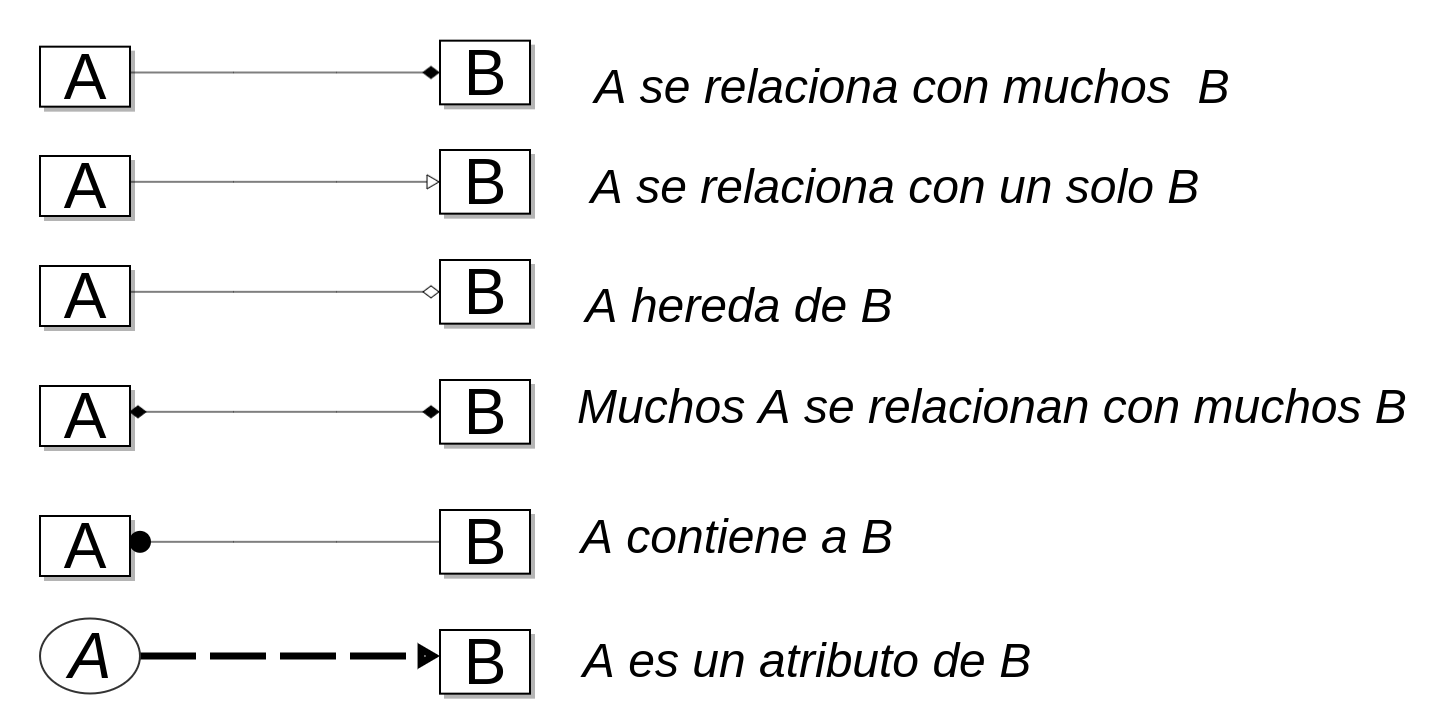
\includegraphics[width=1\linewidth]{images/Introduction/style_conventions}
	\caption{Convenciones de estilos}
	\label{fig:style_conventions}
\end{figure}
	
	

%\end{introduction}
